\section{Version control systems and Git history}

\begin{frame}
\frametitle{What are Version Control Systems?}
\begin{itemize}

    \item A way to track changes\footnote[frame]{e.g. when, what, by whom,
        and why} to groups of files
    \item Most often used in software projects
    \item Most often used to track changes to text files (but not
        exclusively)
\end{itemize}
\end{frame}

\begin{frame}[fragile]
\frametitle{What are Version Control Systems?}
\begin{itemize}
    \item Akin to a time machine: one can return to previous states of a
        project
\end{itemize}
\begin{figure}
    \centerline{%
    \includegraphics[width=0.7\textwidth]{images/The_Delorian_William_Warby_flickr.pdf}}
        \caption{\tiny \emph{The Delorian}, by William Warby, Flickr:
    \url{https://www.flickr.com/photos/wwarby/9641216546/in/photostream/}}
\end{figure}
\end{frame}

\begin{frame}[fragile]
\frametitle{What are Version Control Systems?}
    \begin{itemize}
        \item Like a safety net: accidental file deletion isn't a catastrophe
    \end{itemize}
    \begin{figure}
        \centerline{%
            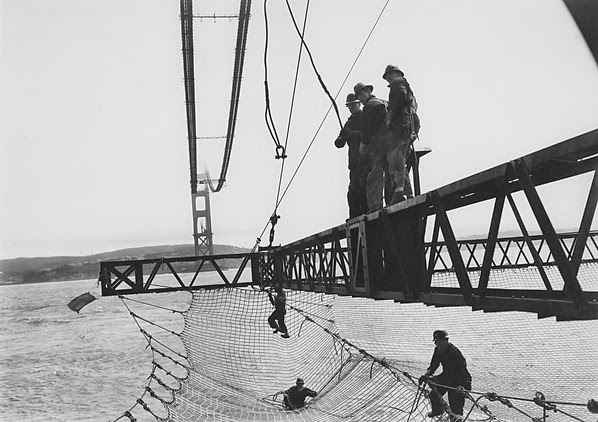
\includegraphics[height=0.65\textheight]{images/safety_net_golden_gate_bridge.jpg}}
            \caption{\tiny \url{https://todayinlaborhistory.wordpress.com/2015/01/05/january-5-1933/}}
    \end{figure}

\end{frame}

\begin{frame}[fragile]
\frametitle{What are Version Control Systems?}
    \begin{multicols}{2}
        \begin{itemize}
            \item Saved states are like anchor points in like rock climbing:
                one can fall back a small distance without losing everything
        \end{itemize}
        \begin{figure}
            \centerline{%
                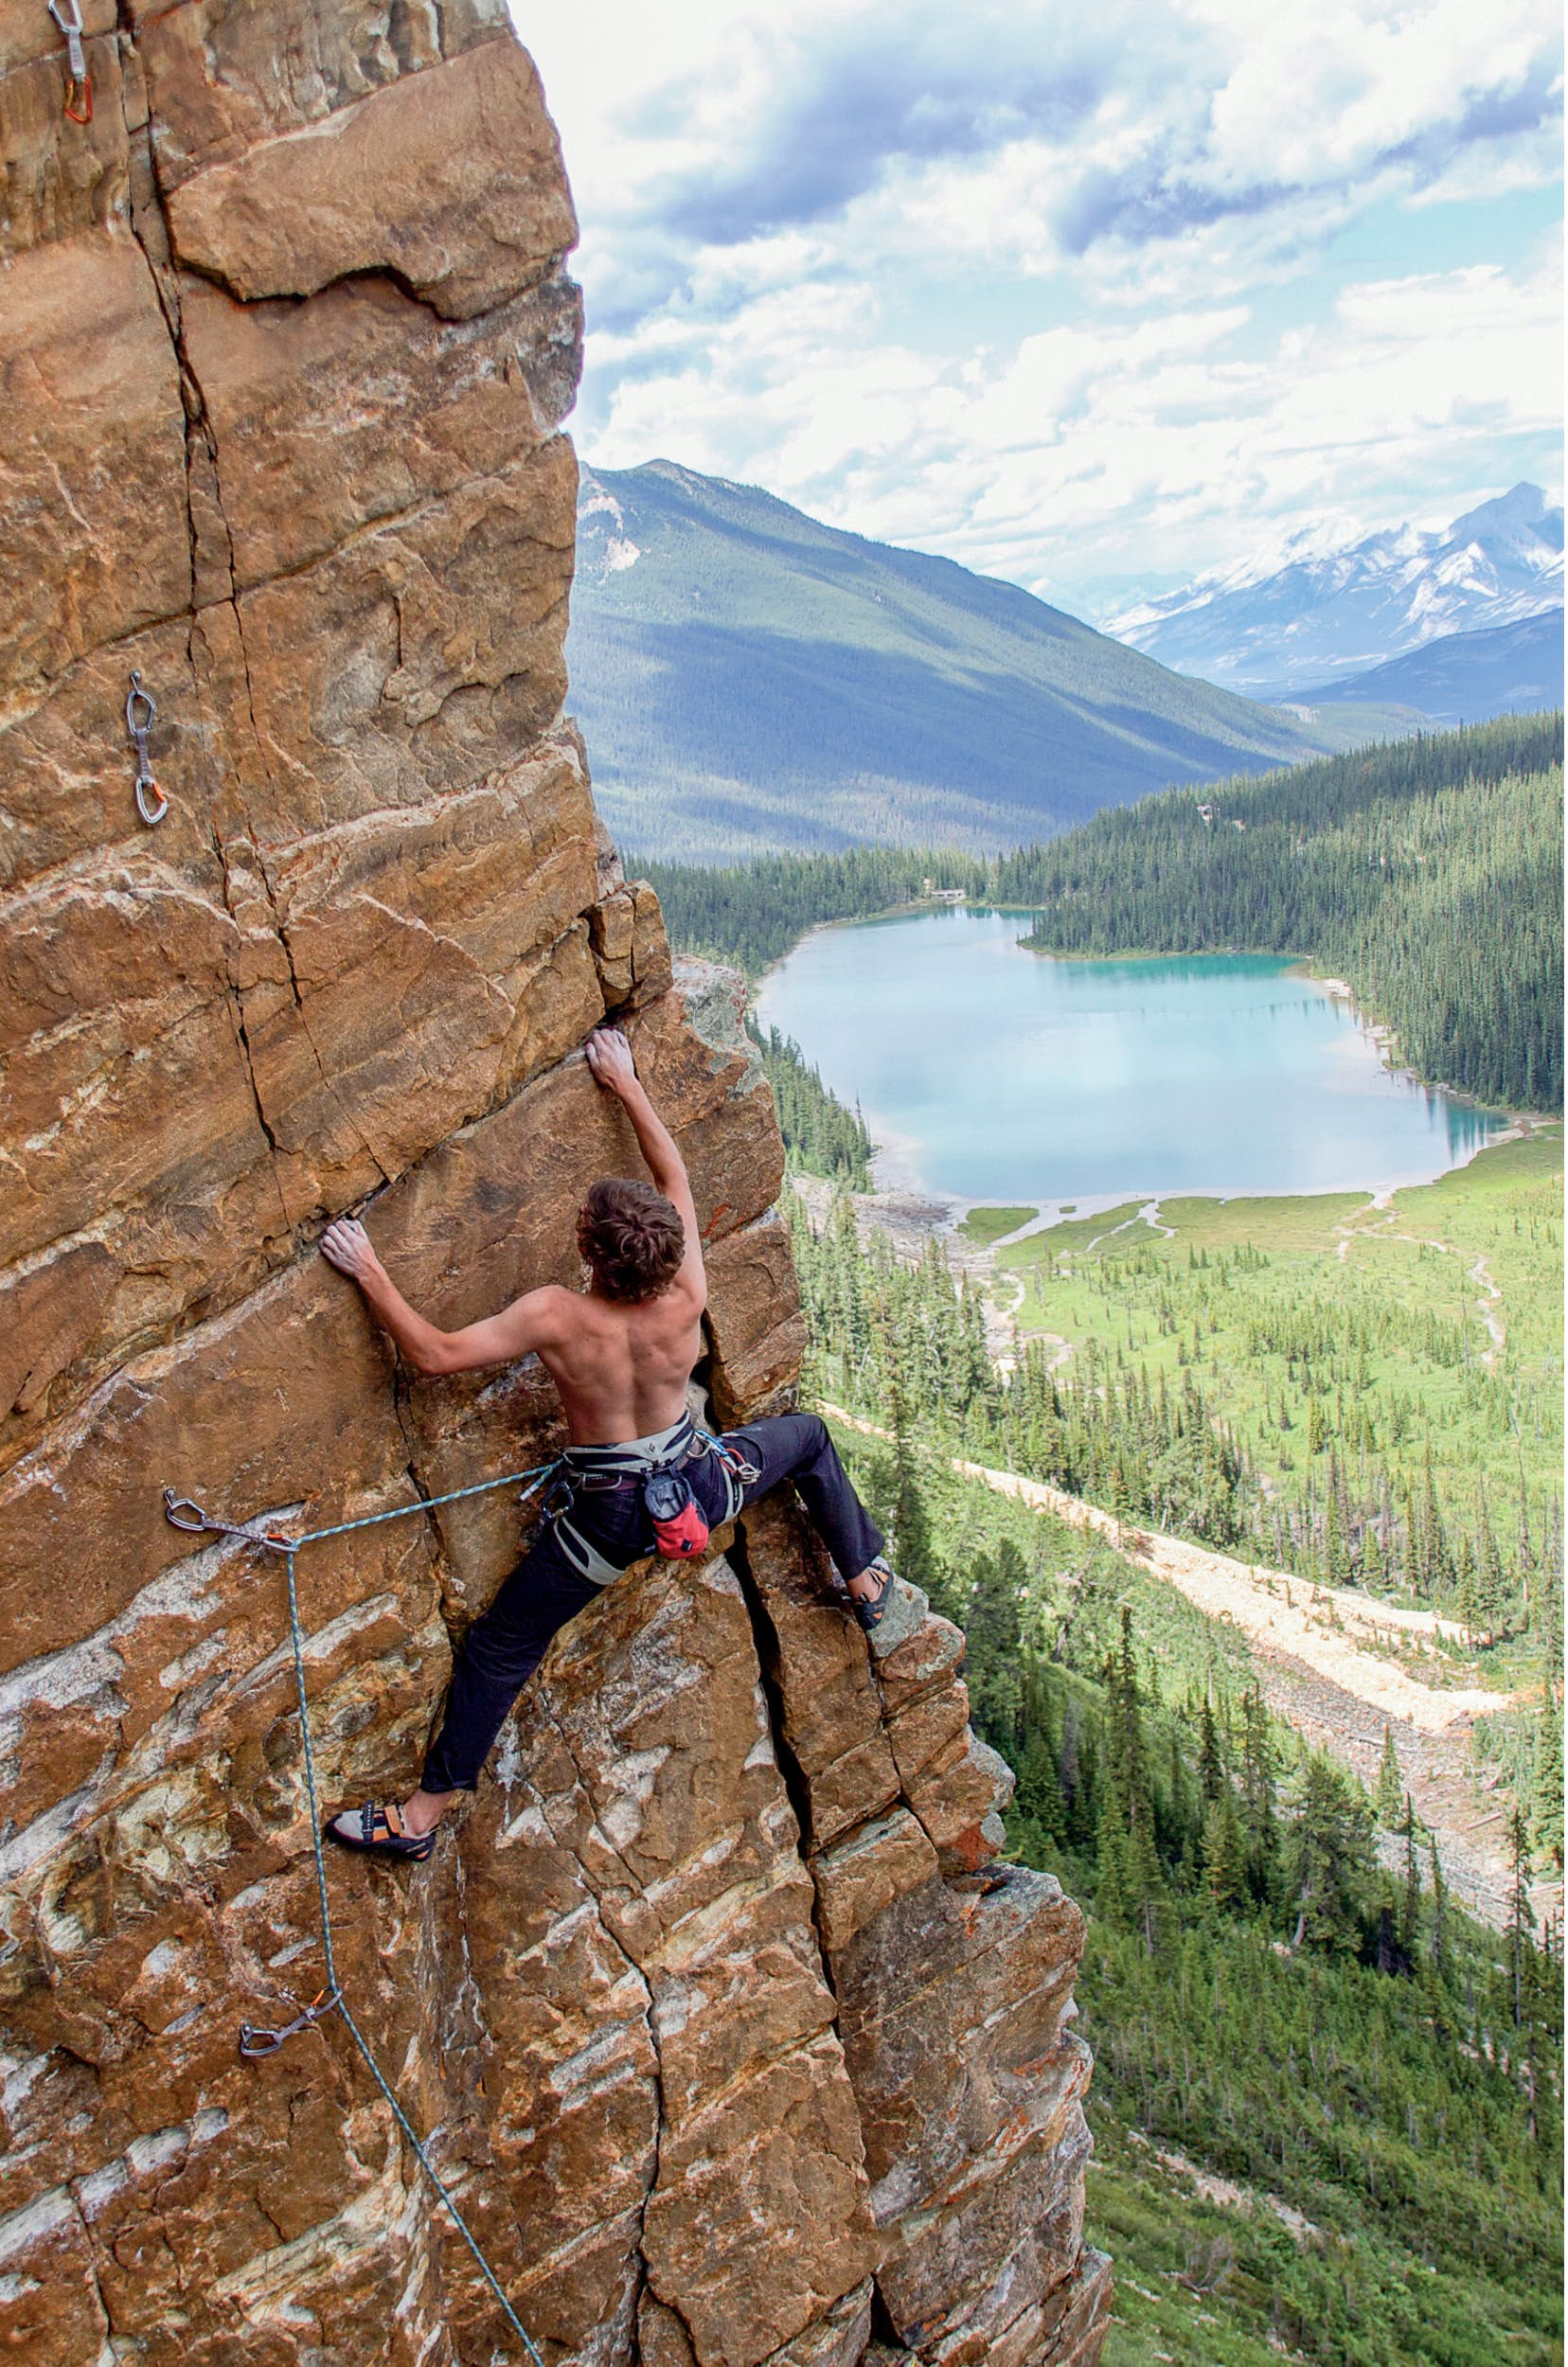
\includegraphics[height=0.8\textheight]{images/northern_exposure_jasper_rock_climbing.jpg}}
                \caption{\tiny by Fran\c{c}ois Laplante, \url{http://www.northernexposurejasper.com/}}
        \end{figure}
    \end{multicols}
\end{frame}

\begin{frame}[fragile]
\frametitle{Why use a Version Control System?}

Does this look familiar?

\begin{lstlisting}
$ ls
file.1      file.20090803  file.keep
file.2      file.alt       file.old
file.old.2  file.fixed     file.new
\end{lstlisting}
%stopzone

This is better than nothing, however \ldots
\begin{itemize}
    \item what happened between the different versions?  And just as
        important: \emph{why}?
    \item which file is actually the most current?
    \item what if \ttt{file.old} is the \emph{newest} file?
    \item can the differences between files tell us anything?
    \item why store \emph{nine} files when we really only need one?
\end{itemize}
\end{frame}

\begin{frame}
\frametitle{Why use a Version Control System?}
\begin{itemize}
    \item Version Control Systems help to tame this chaos
    \item Useful in detecting when bugs were introduced or fixed
    \item Used to save known states of a group of files and hence versions
        (releases) of a software project
    \item Can aid work on collaborative projects
\end{itemize}
\end{frame}

\begin{frame}
\frametitle{Version Control Systems: Local Model}
        % -> image/diagram of local system
\begin{itemize}
    \item Restricted to a single computer
    \item Historically also only able to be used by one person at a time
        (e.g. access control via file locking)
    \item Examples:
        \begin{itemize}
            \item \href{https://en.wikipedia.org/wiki/Revision_Control_System}
                       {Revision Control System (RCS)}
            \item \href{https://en.wikipedia.org/wiki/Source_Code_Control_System}
                       {Source Code Control System (SCCS)}
        \end{itemize}
\end{itemize}
\end{frame}

\begin{frame}[fragile]
\frametitle{Version Control Systems: Centralised Model}
\begin{columns}[T]
    \begin{column}{0.7\textwidth}
        \begin{itemize}
            \item Client-Server architecture
            \item Server contains all repository files and is ``single source of truth''
            \item Clients contain copies of repository, where one work on project
                files (\emph{working copy})
            \item Require network access to server for version control actions
            \item Examples:
            \begin{itemize}
                \item \href{https://en.wikipedia.org/wiki/Concurrent_Versions_System}
                           {Concurrent Versions System (CVS)}
                \item \href{https://en.wikipedia.org/wiki/Apache_Subversion}
                           {Subversion (SVN)}
            \end{itemize}
        \end{itemize}
    \end{column}
    \begin{column}{0.4\textwidth}
        \begin{center}
        \resizebox{\textwidth}{!}{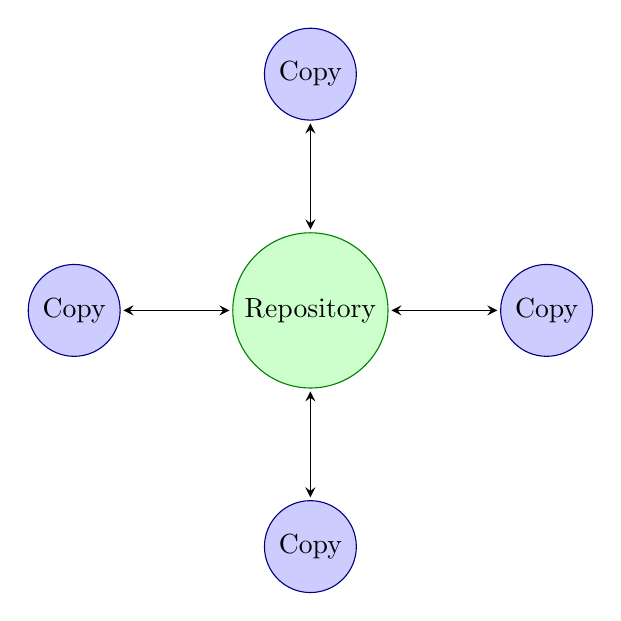
\begin{tikzpicture}
[repo/.style={circle,
		fill=green!20!white,
		draw=green!50!black,
		minimum size=10mm},
workingcopy/.style={circle,
		fill=blue!20!white,
		draw=blue!50!black,
		minimum size=5mm},
link/.style={<->, shorten <=1pt, shorten >=1pt, >=stealth, semithick}]

% central repo
\node at (0, 0) [repo] (mainrepo) { Repository };
% working copies
\node at (3,0)  [workingcopy] (copyright)  { Copy };
\node at (-3,0) [workingcopy] (copyleft)   { Copy };
\node at (0,3)  [workingcopy] (copytop)    { Copy };
\node at (0,-3) [workingcopy] (copybottom) { Copy };
% links between repo and working copies
\draw [link] (mainrepo) -- (copyright);
\draw [link] (mainrepo) -- (copyleft);
\draw [link] (mainrepo) -- (copytop);
\draw [link] (mainrepo) -- (copybottom);
\end{tikzpicture}
}
        \end{center}
    \end{column}
\end{columns}
\end{frame}

\begin{frame}
\frametitle{Version Control Systems: Distributed Model}
        % -> image/diagram of distributed system
\begin{itemize}
    \item Client-Server or Peer-to-peer or a mixture of the two
    \item Each client has complete repository and its entire history
    \item Server no longer strictly required; if used, contains a ``bare''
        version of the repository, i.e. the working directory is not present
    \item Offline work now possible and simple
    \item When collaborating can resync work when online again
    \item Examples:
        \begin{itemize}
            \item \href{https://git-scm.com/}{Git}
                
\includegraphics[height=0.05\textheight]{images/git_logo.png}
            \item \href{https://www.mercurial-scm.org/}{Mercurial}
                
\includegraphics[height=0.05\textheight]{images/mercurial_logo.png}
        \end{itemize}
\end{itemize}
\end{frame}

\begin{frame}
\frametitle{A short Git History}
\begin{itemize}
    \item Linux kernel development could use proprietary BitKeeper system
        free of charge
    \item The owners of BitKeeper changed the licensing conditions, which
        meant that it was no longer free for kernel developers to use
    \item Thus Linus Torvalds wrote his own system: Git
    \item Open source with a large developer community and an even larger
        user base.
\end{itemize}
\end{frame}

\begin{frame}
    \frametitle{Why use Git?}
    \begin{itemize}
        \item Supports distributed development
        \item Doesn't rely on network availability
        \item Scales to thousands of developers and millions of commits
        \item Fast!
        \item Repositories contain complete project history
        \item Lightweight branches
        \item Atomic operations
        \item Open source
        \item Free as in freedom
    \end{itemize}
\end{frame}

% vim: expandtab shiftwidth=4 softtabstop=4
